\documentclass[a4paper,11pt]{report}
\usepackage{chuan_math_gkt}
\usetikzlibrary{angles,quotes,intersections,patterns,decorations.pathreplacing}
\chuanexamsetup

\begin{document}
\examfontsize

\examsecret{绝密$\bigstar$启用前}

\examtitle{2022年普通高等学校招生全国统一考试（全国甲卷文科）}{数\quad 学}

\noticetitle
\begin{examnotice}
\item 答卷前，考生务必将自己的姓名、准考证号填写在答题卡上. 
\item 回答选择题时，选出每小题的答案后，用铅笔把答题卡上对应题目的答案标号涂黑. 如需改动，用橡皮擦干净后，再选涂其他答案标号. 回答非选择题时，将答案写在答题卡上. 写在本试卷上无效. 
\item 考试结束后，将本试卷和答题卡一并交回. 
\end{examnotice}

\examsection{一、选择题：本题共12小题，每小题5分，共60分. 在每小题给出的四个选项中，只有一项是符合题目要求的. }
\begin{examquestions}
\item 设集合 $A=\{-2,-1,0,1,2\}$，$B=\left\{x\mid 0\leq x<\dfrac52\right\}$，则 $A\cap B=$
\fourchoices{$\{0,1,2\}$}{$\{-2,-1,0\}$}{$\{0,1\}$}{$\{1,2\}$}
\item 某社区通过公益讲座以普及社区居民垃圾分类知识. 为了解讲座效果，随机抽取10位社区居民，让他们在讲座前和讲座后各回答一份垃圾分类知识问卷，这10位社区居民在讲座前和讲座后问卷答题的正确率如下图：
\begin{tightcenter}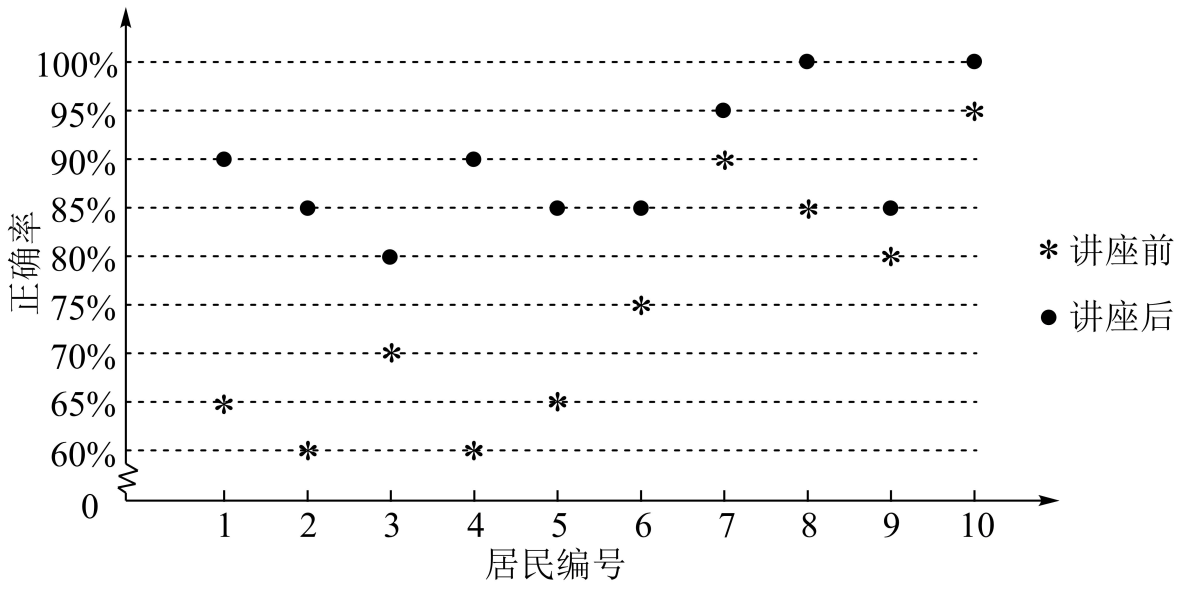
\includegraphics[width=10.5cm]{figures/2022_jiawen_q2.png}\end{tightcenter}
则
\onechoices{讲座前问卷答题的正确率的中位数小于 $70\%$}{讲座后问卷答题的正确率的平均数大于 $85\%$}{讲座前问卷答题的正确率的标准差小于讲座后正确率的标准差}{讲座后问卷答题的正确率的极差大于讲座前正确率的极差}
\item 若 $z=1-\sqrt3\mathrm{i}$，则 $|z|=$
\fourchoices{$4$}{$4\sqrt2$}{$2\sqrt5$}{$2\sqrt2$}

\begin{minipage}[t]{0.66\linewidth}
\item 如图，网格纸上绘制的是一个多面体的三视图，网格小正方形的边长为1，则该多面体的体积为
\vspace{0.5em}
\twochoices{$8$}{$12$}{$16$}{$20$}

\end{minipage}\hfill
\begin{minipage}[t]{0.3\linewidth}
\vspace{0em}\centering
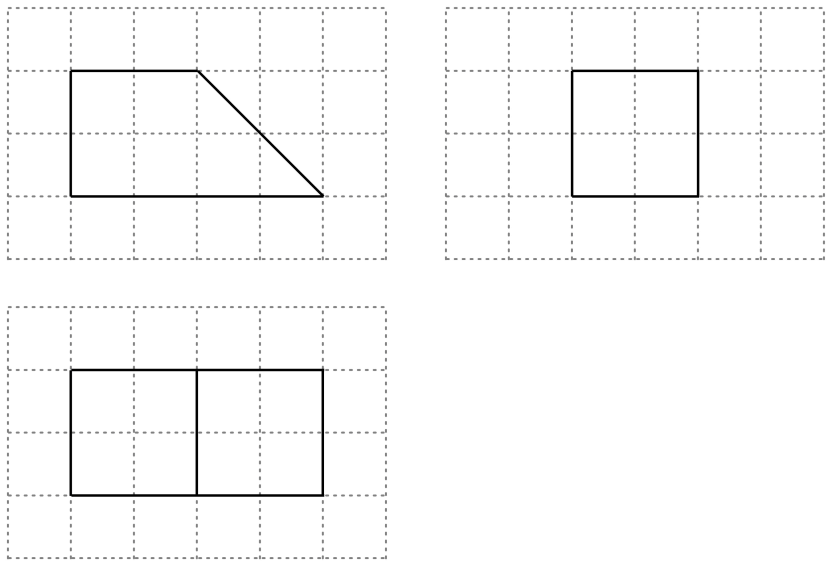
\includegraphics[width=\linewidth]{figures/2022_jiali_q4.png}
\end{minipage}
\vspace{-0.5em}
\item 将函数 $y=\sin\left(\omega x+\dfrac\pi3\right)(\omega>0)$ 的图像向左平移 $\dfrac\pi{12}$ 个单位长度后得到曲线 $C$，若 $C$ 关于 $y$ 轴对称，则 $\omega$ 的最小值是
\fourchoices{\tallchoice{$\dfrac16$}}{\tallchoice{$\dfrac14$}}{\tallchoice{$\dfrac13$}}{\tallchoice{$\dfrac12$}}
\item 从分别写有1，2，3，4，5，6的6张卡片中无放回随机抽取2张，则抽到的2张卡片上的数字之积是4的倍数的概率为
\fourchoices{\tallchoice{$\dfrac15$}}{\tallchoice{$\dfrac13$}}{\tallchoice{$\dfrac25$}}{\tallchoice{$\dfrac23$}}
\item 函数 $y=(3^x-3^{-x})\cos x$ 在区间 $\left[-\dfrac\pi2,\dfrac\pi2\right]$ 的图象大致为
\graphchoicesoneline
{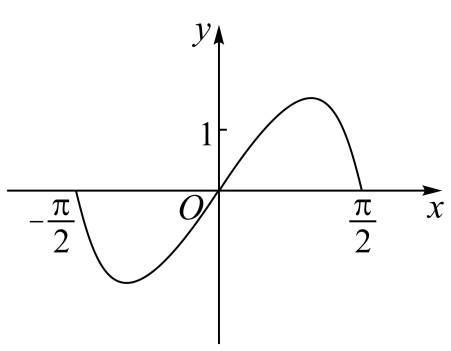
\includegraphics[width=2.7cm]{figures/2022_jiali_q5_A.png}}
{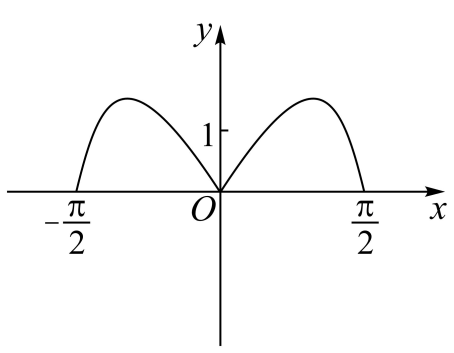
\includegraphics[width=2.7cm]{figures/2022_jiali_q5_B.png}}
{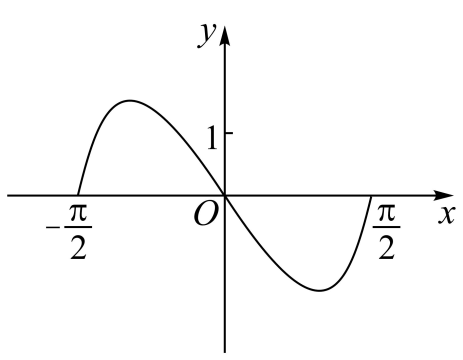
\includegraphics[width=2.7cm]{figures/2022_jiali_q5_C.png}}
{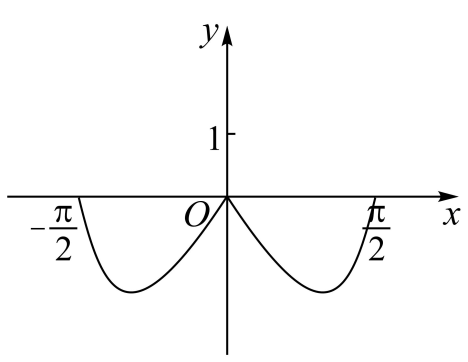
\includegraphics[width=2.7cm]{figures/2022_jiali_q5_D.png}}

\item 当 $x=1$ 时，函数 $f(x)=a\ln x+\dfrac bx$ 取得最大值 $-2$，则 $f'(2)=$
\fourchoices{$-1$}{{$-\dfrac12$}}{{$\dfrac12$}}{$1$}
\item 在长方体 $ABCD-A_1B_1C_1D_1$ 中，已知 $B_1D$ 与平面 $ABCD$ 和平面 $AA_1B_1B$ 所成的角均为 $30^\circ$，则
\twochoices{$AB=2AD$}{$AB$ 与平面 $AB_1C_1D$ 所成的角为 $30^\circ$}{$AC=CB_1$}{$B_1D$ 与平面 $BB_1C_1C$ 所成的角为 $45^\circ$}
\item 甲、乙两个圆锥的母线长相等，侧面展开图的圆心角之和为 $2\pi$，侧面积分别为 $S_\text{甲}$ 和 $S_\text{乙}$，体积分别为 $V_\text{甲}$ 和 $V_\text{乙}$. 若 $\dfrac{S_\text{甲}}{S_\text{乙}}=2$，则 $\dfrac{V_\text{甲}}{V_\text{乙}}=$
\fourchoices{$\sqrt5$}{$2\sqrt2$}{$\sqrt{10}$}{{$\dfrac{5\sqrt{10}}{4}$}}
\vspace{-0.4em}
\item 已知椭圆 $C:\dfrac{x^2}{a^2}+\dfrac{y^2}{b^2}=1(a>b>0)$ 的离心率为 $\dfrac12$，$A_1,A_2$ 分别为 $C$ 的左、右顶点，$B$ 为 $C$ 的上顶点. 若 $\overrightarrow{BA_1}\cdot\overrightarrow{BA_2}=-1$，则 $C$ 的方程为
\fourchoices{\tallchoice{$\dfrac{x^2}{18}+\dfrac{y^2}{16}=1$}}{\tallchoice{$\dfrac{x^2}{8}+\dfrac{y^2}{4}=1$}}{\tallchoice{$\dfrac{x^2}{3}+\dfrac{y^2}{2}=1$}}{\tallchoice{$\dfrac{x^2}{2}+y^2=1$}}
\item 已知 $a=\dfrac{31}{32}$，$b=\cos\dfrac14$，$c=4\sin\dfrac14$，则
\fourchoices{$a>b>c$}{$a>c>b$}{$c>b>a$}{$b>c>a$}
\end{examquestions}
\examsection{二、填空题：本题共4小题，每小题5分，共20分. }
\begin{examquestions}[start=13]
\item 已知向量 $\vec a=(m,1)$，$\vec b=(1,2)$. 若 $\vec a\parallel\vec b$，则 $m=\blank$. 
\item 设点 $M$ 在直线 $2x+y-1=0$ 上，点 $(3,0)$ 和 $(0,1)$ 均在圆 $C$ 上，则 $C$ 的方程为\blank. 
\item 记双曲线 $C:\dfrac{x^2}{a^2}-\dfrac{y^2}{b^2}=1(a>0,b>0)$ 的离心率为 $e$，写出满足条件“直线 $y=2x$ 与 $C$ 无公共点”的 $e$ 的一个值\blank. 
\item 已知 $\triangle ABC$ 中，点 $D$ 在边 $BC$ 上，$\angle ADB=120^\circ$，$AD=2$，$CD=2BD$. 当 $\dfrac{AC}{AB}$ 取得最小值时，$BD=\blank$. 
\end{examquestions}
\examsection{三、解答题：共70分. 解答应写出文字说明、证明过程或演算步骤. 第17题～第21题为必考题，每个试题考生都必须作答. 第22、23题为选考题，考生根据要求作答. }
\begin{examanswers}[start=17]
\item（12分）

甲、乙两城之间的长途客车均由A和B两家公司运营，为了解这两家公司长途客车的运行情况，随机调查了甲、乙两城之间的500个班次，得到下面列联表：
\begin{tightcenter}
{\renewcommand{\arraystretch}{0.9}
    \begin{tabular}{|c|c|c|}\hline & 准点班次数 & 未准点班次数\\ \hline A & 240 & 20\\ \hline B & 210 & 30\\ \hline\end{tabular}}\end{tightcenter}
\subq{（1）}{根据上表，分别估计这两家公司甲、乙两城之间的长途客车准点的概率；}

\subq{（2）}{能否有90\%把握认为甲、乙两城之间的长途客车是否准点与客车所属公司有关？
附：$K^2=\dfrac{n(ad-bc)^2}{(a+b)(c+d)(a+c)(b+d)}$. 
\begin{tightcenter}    {\renewcommand{\arraystretch}{0.9}\begin{tabular}{|c|c|c|c|}\hline $P(K^2\geq k)$ & 0.100 & 0.050 & 0.010\\ \hline $k$ & 2.706 & 3.841 & 6.635\\ \hline\end{tabular}}\end{tightcenter}
}
\item（12分）

记 $S_n$ 为数列 $\{a_n\}$ 的前 $n$ 项和. 已知 $\dfrac{2S_n}{n}+n=2a_n+1$. 

\subq{（1）}{证明：$\{a_n\}$ 是等差数列；}

\subq{（2）}{若 $a_4,a_7,a_9$ 成等比数列，求 $S_n$ 的最小值.}

\newpage
\item（12分）

小明同学参加综合实践活动，设计了一个封闭的包装盒，包装盒如图所示：底面 $ABCD$ 是边长为8（单位：$\mathrm{cm}$）的正方形，$EAB,FBC,GCD,HDA$ 均为正三角形，且它们所在的平面都与平面 $ABCD$ 垂直. 

\noindent\begin{minipage}[t]{0.62\linewidth}
\subq{（1）}{证明：$EF\parallel$ 平面 $ABCD$；}

\subq{（2）}{求该包装盒的容积（不计包装盒材料的厚度）.}
\end{minipage}\hfill
\begin{minipage}[t]{0.26\linewidth}\vspace{-2em}\centering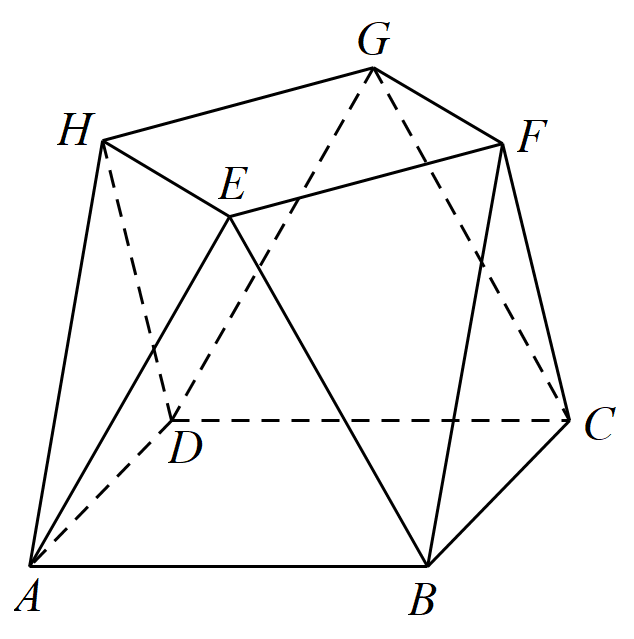
\includegraphics[width=\linewidth]{figures/2022_jiawen_q19.png}\end{minipage}
\vspace{-3em}
\item（12分）

已知函数 $f(x)=x^3-x,g(x)=x^2+a$，曲线 $y=f(x)$ 在点 $(x_1,f(x_1))$ 处的切线也是曲线 $y=g(x)$ 的切线. 

\subq{（1）}{若 $x_1=-1$，求 $a$；}

\subq{（2）}{求 $a$ 的取值范围.}
\vspace{-0.5em}
\item（12分）

设抛物线 $C:y^2=2px(p>0)$ 的焦点为 $F$，点 $D(p,0)$，过 $F$ 的直线交 $C$ 于 $M,N$ 两点. 当直线 $MD$ 垂直于 $x$ 轴时，$|MF|=3$. 

\subq{（1）}{求 $C$ 的方程；}

\subq{（2）}{设直线 $MD,ND$ 与 $C$ 的另一个交点分别为 $A,B$，记直线 $MN,AB$ 的倾斜角分别为 $\alpha,\beta$. 当 $\alpha-\beta$ 取得最大值时，求直线 $AB$ 的方程.}
\end{examanswers}


\begin{examanswers}[start=22]
\item（10分）【选修4-4：坐标系与参数方程】

在直角坐标系 $xOy$ 中，曲线 $C_1$ 的参数方程为\linsys{x=\dfrac{2+t}{6},\\ y=\sqrt t}（$t$ 为参数），曲线 $C_2$ 的参数方程为\linsys{x=-\dfrac{2+s}{6},\\ y=-\sqrt s}（$s$ 为参数）. 

\subq{（1）}{写出 $C_1$ 的普通方程；}

\subq{（2）}{以坐标原点为极点，$x$ 轴正半轴为极轴建立极坐标系，曲线 $C_3$ 的极坐标方程为 $2\cos\theta-\sin\theta=0$，求 $C_3$ 与 $C_1$ 交点的直角坐标，及 $C_3$ 与 $C_2$ 交点的直角坐标.}
\vspace{-0.5em}
\item（10分）【选修4-5：不等式选讲】

已知 $a,b,c$ 均为正数，且 $a^2+b^2+4c^2=3$，证明：

\subq{（1）}{$a+b+2c\leq3$；}

\subq{（2）}{若 $b=2c$，则 $\dfrac1a+\dfrac1c\geq3$.}
\end{examanswers}

\end{document}
